% Options for packages loaded elsewhere
\PassOptionsToPackage{unicode}{hyperref}
\PassOptionsToPackage{hyphens}{url}
%
\documentclass[
  11pt,
]{article}
\usepackage{amsmath,amssymb}
\usepackage{iftex}
\ifPDFTeX
  \usepackage[T1]{fontenc}
  \usepackage[utf8]{inputenc}
  \usepackage{textcomp} % provide euro and other symbols
\else % if luatex or xetex
  \usepackage{unicode-math} % this also loads fontspec
  \defaultfontfeatures{Scale=MatchLowercase}
  \defaultfontfeatures[\rmfamily]{Ligatures=TeX,Scale=1}
\fi
\usepackage{lmodern}
\ifPDFTeX\else
  % xetex/luatex font selection
\fi
% Use upquote if available, for straight quotes in verbatim environments
\IfFileExists{upquote.sty}{\usepackage{upquote}}{}
\IfFileExists{microtype.sty}{% use microtype if available
  \usepackage[]{microtype}
  \UseMicrotypeSet[protrusion]{basicmath} % disable protrusion for tt fonts
}{}
\makeatletter
\@ifundefined{KOMAClassName}{% if non-KOMA class
  \IfFileExists{parskip.sty}{%
    \usepackage{parskip}
  }{% else
    \setlength{\parindent}{0pt}
    \setlength{\parskip}{6pt plus 2pt minus 1pt}}
}{% if KOMA class
  \KOMAoptions{parskip=half}}
\makeatother
\usepackage{xcolor}
\usepackage[a4paper, top=12mm, bottom=15mm]{geometry}
\usepackage{longtable,booktabs,array}
\usepackage{calc} % for calculating minipage widths
% Correct order of tables after \paragraph or \subparagraph
\usepackage{etoolbox}
\makeatletter
\patchcmd\longtable{\par}{\if@noskipsec\mbox{}\fi\par}{}{}
\makeatother
% Allow footnotes in longtable head/foot
\IfFileExists{footnotehyper.sty}{\usepackage{footnotehyper}}{\usepackage{footnote}}
\makesavenoteenv{longtable}
\usepackage{graphicx}
\makeatletter
\def\maxwidth{\ifdim\Gin@nat@width>\linewidth\linewidth\else\Gin@nat@width\fi}
\def\maxheight{\ifdim\Gin@nat@height>\textheight\textheight\else\Gin@nat@height\fi}
\makeatother
% Scale images if necessary, so that they will not overflow the page
% margins by default, and it is still possible to overwrite the defaults
% using explicit options in \includegraphics[width, height, ...]{}
\setkeys{Gin}{width=\maxwidth,height=\maxheight,keepaspectratio}
% Set default figure placement to htbp
\makeatletter
\def\fps@figure{htbp}
\makeatother
\setlength{\emergencystretch}{3em} % prevent overfull lines
\providecommand{\tightlist}{%
  \setlength{\itemsep}{0pt}\setlength{\parskip}{0pt}}
\setcounter{secnumdepth}{5}
\usepackage{booktabs}
\usepackage{longtable}
\usepackage{array}
\usepackage{multirow}
\usepackage{wrapfig}
\usepackage{float}
\usepackage{colortbl}
\usepackage{pdflscape}
\usepackage{tabu}
\usepackage{threeparttable}
\usepackage{threeparttablex}
\usepackage[normalem]{ulem}
\usepackage{makecell}
\usepackage{xcolor}
\ifLuaTeX
  \usepackage{selnolig}  % disable illegal ligatures
\fi
\usepackage{bookmark}
\IfFileExists{xurl.sty}{\usepackage{xurl}}{} % add URL line breaks if available
\urlstyle{same}
\hypersetup{
  pdftitle={Replication of DistilBERT evaluation results},
  hidelinks,
  pdfcreator={LaTeX via pandoc}}

\title{Replication of DistilBERT evaluation results}
\author{Group M - Nadun Chandrabahu, Vu Anh Tai Ho\\
Thanushreyas Appaji, Muhammad Umer Bashir}
\date{November 1, 2024}

\begin{document}
\maketitle

\section{Introduction}\label{introduction}

Reproducible research is vital in machine learning for several reasons.
Firstly, it enables the validation of results, when research can be
consistently reproduced, it enhances the credibility of the original
findings. Additionally, reproducibility supports benchmarking for
comparing algorithms and models, allowing the machine learning community
to identify the best-performing models. It also plays an important role
in identifying errors and biases, such as coding mistakes or data
handling issues, improving the reliability of the research.

The paper that we selected for this project, (Sanh et al,
2019)\footnote{(Sanh et al, 2019):
  \url{https://arxiv.org/pdf/1910.01108}} ``DistilBERT, a distilled
version of BERT: smaller, faster, cheaper and lighter'', presents a
method for training a more compact general-purpose language
representation model called DistilBERT, which is a streamlined version
of the larger BERT model (Bidirectional Encoder Representations from
Transformers). Although BERT is highly effective for Natural Language
Processing (NLP) tasks, its size and complexity can lead to slower
inference times, particularly in on-the-edge or resource-constrained
environments, potentially impacting user experience. This paper aims to
pre-train the DistilBERT model to enhance inference performance by
reducing both its size and inference time while maintaining accuracy.
According to the paper, DistilBERT achieves a 40\% reduction in model
size, preserves 97\% of BERT's language understanding capabilities, and
improves processing speed by 60\%.

The source files and collaborative work done on this project is
available for review on GitHub\footnote{Project on GitHub:
  \url{https://github.com/nadunchandrabahu/COMP8240-GroupM}}.

\section{Project Justification}\label{project-justification}

In this project, we will not replicate the transfer learning or model
training processes of DistilBERT. Instead, we aim to reproduce the
evaluation metrics shown in Tables 1 and 2 on page 3 of the referenced
research paper, across various datasets and downstream tasks. This will
allow us to assess DistilBERT's performance both on the datasets from
the paper and on some of our own datasets. The DistilBERT model is
available for evaluation through Hugging Face's transformers library
(Wolf et al., 2019). In the original research, DistilBERT was evaluated
using three datasets: the GLUE (General Language Understanding and
Evaluation)\footnote{GLUE Benchmark: \url{https://gluebenchmark.com/}}
benchmark, which includes nine sentence-pair language understanding
tasks; IMDb (Internet Movie Database)\footnote{IMDb dataset:
  \url{https://www.kaggle.com/datasets/lakshmi25npathi/imdb-dataset-of-50k-movie-reviews}},
used for sentiment classification of user movie reviews; and SQuAD
(Stanford Question Answering Dataset)\footnote{SQuAD v1.1 dataset:
  \url{https://rajpurkar.github.io/SQuAD-explorer/}}, designed for
question-answering based on a provided context.

We will run some python code on Jupyter/Colab notebooks to make
predictions on the data with the DistilBERT model and calculate various
metrics: the average score across the nine GLUE benchmark tasks, test
accuracy on the IMDb dataset, and the Exact Match (EM) and F1 score on
the SQuAD task. These metrics are reported in Tables 1 and 2 of the
research paper and it is the aim of this project to replicate these
results. Each group member will also show the metrics using new data
sources to perform similar NLP tasks with DistilBERT.

Table 1 below shows the scoring of DistilBERT evaluation on 9 GLUE
benchmark tasks as shown in the research paper.

\begin{longtable}[t]{ccccccccccc}
\caption{\label{tab:table1}BERT and DistilBERT results on GLUE tasks}\\
\toprule
\multicolumn{1}{c}{ } & \multicolumn{10}{c}{Metrics} \\
\cmidrule(l{3pt}r{3pt}){2-11}
Model.Name & Score & CoLA & MNLI & MRPC & QNLI & QQP & RTE & SST.2 & STS.B & WNLI\\
\midrule
 &  &  &  &  &  &  &  &  &  & \\
BERT-base & 79.5 & 56.3 & 86.7 & 88.6 & 91.8 & 89.6 & 69.3 & 92.7 & 89 & 53.5\\
DistilBERT & 77 & 51.3 & 82.2 & 87.5 & 89.2 & 88.5 & 59.9 & 91.3 & 86.9 & 56.3\\
\bottomrule
\end{longtable}

Table 2 below shows the test accuracy of IMDb sentiment analysis tasks,
and EM/F1 scores of the SQuAD question answering task as shown on the
research paper.

\begin{longtable}[t]{cccc}
\caption{\label{tab:table2}IMDb and SQuAD metrics}\\
\toprule
\multicolumn{1}{c}{ } & \multicolumn{1}{c}{IMDb} & \multicolumn{2}{c}{SQuAD} \\
\cmidrule(l{3pt}r{3pt}){2-2} \cmidrule(l{3pt}r{3pt}){3-4}
Model Name &  &  & \\
\midrule
 & acc. & EM & F1\\
BERT-base & 93.46 & 81.2 & 88.5\\
DistilBERT & 92.82 & 77.7 & 85.8\\
\bottomrule
\end{longtable}

\section{Original Datasets}\label{original-datasets}

\subsection{GLUE Benchmark}\label{glue-benchmark}

GLUE (General Language Understanding Evaluation) contains 9 tasks from
sentiment understanding to inference to evaluate a Natural Language
Program capability to comprehend and use linguistic effectively compared
to a person with common knowledge.

The 9 tasks are divided on 3 group of tasks: Single-Sentence Tasks,
Similarity and Paraphrase Tasks, and Inference Tasks.

\subsubsection{Single-Sentence Tasks}\label{single-sentence-tasks}

\emph{CoLa} testing linguistic acceptability determining whether a
sentence is grammatically acceptable. It is taken from various piece of
literature and its acceptability is manually marked by verified
linguists \emph{SST-2} testing sentiment understanding by making
predictions whether a sentence is positive or negative. It is sourced
from web movie reviews with binary classification.

\subsubsection{Similarity and Paraprhase
Tasks}\label{similarity-and-paraprhase-tasks}

\emph{MRPC} testing paraphrase capability concerning the news. Microsoft
Research designed this corpus from multiple news sources. It contain
pair of sentences and the label will be judged whether they are similar
or not

\emph{STS-B} testing sentence similarity from a collection of sentences
pair in the domain of news, forums, and image captions. It is a more
fine-grained test when the label are annotated to a float score from 1 -
5. Hence, it uses regression and Pearson correlation coefficients to
evaluate the performance not the usual classification test like the
others

\emph{QQP} testing paraphrase but this time concerning question. It
comes from Quora site containing a pair of questions, the task here is
for NLP model to predict whether the two questions are similar or not

\subsubsection{Natural Language Inference
Tasks}\label{natural-language-inference-tasks}

\emph{MNLI} containing a premise-hypothesis pair about a wide sources of
Fiction, Government Report, Telephone Conversation. The tasks is to test
NLP about generalization to different types of text classified them to
entailment, contradiction, or neutral

\emph{QNLI} also testing a pair but this time question-answer pair. It
comes from Stanford drawing Wikipedia site. The NLP model's task is to
determine whether the answer entail or related to the question

\emph{WNLI} a more challenging test with complex reasoning with data
from fiction books which can be more ambiguous and require commonsense
knowledge and context understanding. The NLP model in this test cannot
simply use cues like pronouns to infer

\emph{RTE} testing textual entailment.The test combines multiple
versions of a challenge dataset (1,2,3,5 to be exact) coming from news
article and Wikipedia. It contains two labels of entailment and not
entailment \#\# IMDb dataset

\subsection{IMDb dataset}\label{imdb-dataset}

(Thanushreyas Appaji) Describe about the dataset. Try to keep section to
about 1/3rd of a page

\subsection{SQuAD dataset}\label{squad-dataset}

The research paper makes use of SQuAD v1.1 development set available on
GitHub\footnote{SQuAD v1.1 Dev set:
  \url{https://github.com/rajpurkar/SQuAD-explorer/tree/master/dataset}}.
The dataset consists of 17968 question-answer combinations. Each
question and answer is based on the provided context. There are multiple
ground truth answers to the same question. We only need to extract the
context, question and answer (answer\_text) for the purpose of
calculating Exact Match and F-Score.

\begin{verbatim}
## Columns of SQuAD devset:
##  ['answer_text', 'answer_start', 'question', 'context', 'subject']
\end{verbatim}

\section{Replication of Evaluation on
Datasets}\label{replication-of-evaluation-on-datasets}

We are able to access the DistilBERT model from `transformers' library
provided by HuggingFace. It is essential to have pyTorch installed
before using the model to make predictions. The amount of time taken to
make predictions depends on the size of the dataset, computational power
and NLP task it tries to achieve.

\subsection{GLUE Benchmark}\label{glue-benchmark-1}

The GLUE Benchmark reevaluation was initiated by Vu Anh Tai Ho using
transformers library together with Trainer method to manage model
training. The datasets are collected directly from HuggingFace's
datasets library. Then tokenized using DistilBertTokenizerFast. The
tokenize function are different in the 9 tests just because of the
different format of label and features (some are called sentence1 and
sentence2, some are called premise and hypothesis.

The pretrained-model I used are DistilBertForSequenceClassification for
classification tasks and AutoModelForSequenceClassification for STS-B
task. For simple training process, I use Training Arguments with
settings about epochs, batch size, weight decays, or warmups steps.

The next task is to determine the metrics used to evaluate the
performance of the models. In here I have to use two cases for STS-B
tasks, as the labels are float number, I have to squeeze the predictions
before pass them for pearson correlation coefficients computation in the
metric loaded from datasets library. For other tasks, as label are
ordinal value, I can use argmax to compute the accorded prediction used
in the GLUE Benchmark (accuracy, F1 score, or Matthew's correlation)

\begin{longtable}[]{@{}lccc@{}}
\caption{GLUE Benchmark Results}\tabularnewline
\toprule\noalign{}
Task & Test\_value & Orig\_value & Differences \\
\midrule\noalign{}
\endfirsthead
\toprule\noalign{}
Task & Test\_value & Orig\_value & Differences \\
\midrule\noalign{}
\endhead
\bottomrule\noalign{}
\endlastfoot
cola & 0.43 & 0.51 & 0.08 \\
sst2 & 0.86 & 0.91 & 0.05 \\
mrpc & 0.81 & 0.88 & 0.07 \\
qqp & 0.80 & 0.89 & 0.08 \\
rte & 0.52 & 0.60 & 0.08 \\
wnli & 0.37 & 0.56 & 0.20 \\
stbs & 0.87 & 0.87 & 0.00 \\
mnli & 0.67 & 0.82 & 0.15 \\
\end{longtable}

For the most part, differences are less than 10\% which is acceptable
for using a auto model without much focusing into more complex architect
like using Distilbert inside a neural network architecture with other
Linear classification layer or dropout layer for regularization.
However, the score on wnli and mnli which are inference tasks are not as
good as the original paper, it might due to these model have more
complicated reasoning and context dependence requirement. Therefore, it
might require more complex fine tuning to get to better result.

\subsection{IMDb dataset}\label{imdb-dataset-1}

(Thanushreyas Appaji) Write about how you did the replication. Include
link to notebook

\subsection{SQuAD dataset}\label{squad-dataset-1}

Evaluation of SQuAD (Stanford QUestion Answering Dataset) question
answering task was performed by Nadun Chandrabahu and the
Jupyter-notebook (SQuad-v1.1.ipynb) is available in the github
repository.

Using the DistilBERT model, predicted answers were obtained based on the
context and question. The inference time was 44 minutes on an AMD Ryzen
5 CPU with 16GB RAM. The model prediction returns a score, start and
answer. I made a new column called Exact match that is either 1 or 0 if
the predicted answer is the exact same as the answer\_text column. And I
calculated the average score when the model predicted an exact match. I
obtained a result of 77.6\%, while the research paper reported an EM of
77.7\%.

The F-Score was calculated by using the following formula.

The F-score is given by
\(F1 = 2 \times \frac{\text{Precision} \times \text{Recall}}{\text{Precision} + \text{Recall}}\).

I used the f1\_score function from Python's scikit-learn library to
calculate the F-Score, as well as precision and recall, which rely on
the counts of True Positives, False Positives, and False Negatives. True
Positives occur when the predicted values match the ground truth
exactly. False Positives arise when the prediction overlaps with the
ground truth but is not fully correct, while False Negatives are
predictions that do not align with any part of the ground truth. The
results are visualized in figure 1 below.

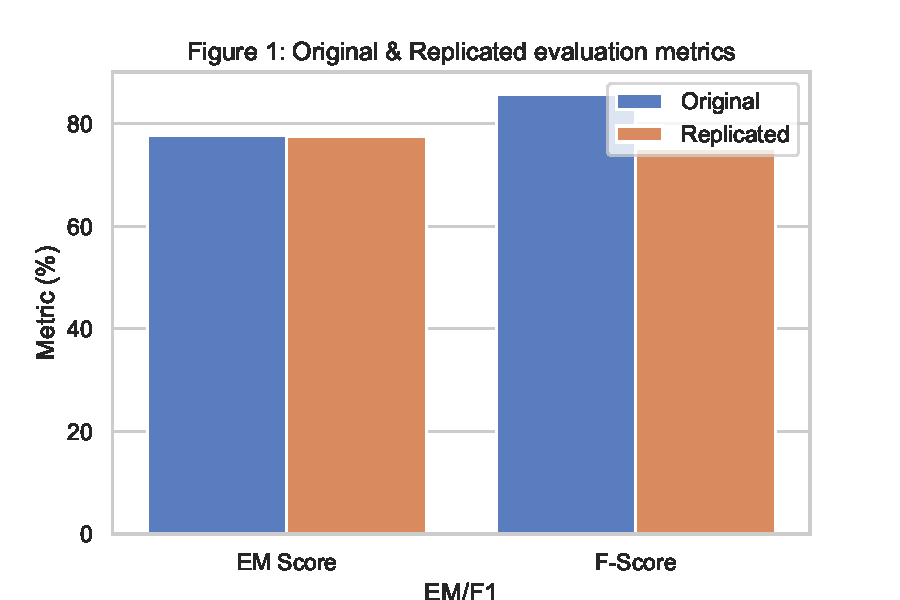
\includegraphics{Final-Report_files/figure-latex/squad_visualization-difference-1.pdf}

As shown in Figure 1, I obtained an F-Score of 75.2\%, which is 10.6\%
lower than the 85.8\% reported in the paper. This difference may stem
from the inherent variability in calculating Precision and Recall, as
the model's predictions can differ slightly with each run, significantly
influencing Precision and Recall values, and hence the F-Score.

\section{Evaluation on New Datasets}\label{evaluation-on-new-datasets}

\subsection{Nadun Chandrabahu}\label{nadun-chandrabahu}

Evaluation of my new dataset McTest (Machine Comprehension
Test)\footnote{McTest Dataset:
  \url{https://huggingface.co/datasets/sagnikrayc/mctest}} (Richardson
et al, 2013) with question answering task was performed and the
Jupyter-notebook (own-dataset.ipynb) is available in the github
repository.

The dataset includes 600 records of the following columns:

\begin{verbatim}
## Columns of McTest devset:
##  idx, question, story,
## properties, answer_options, answer, question_is_multiple
\end{verbatim}

The dataset can be easily loaded into Python using the
\texttt{load\_datasets} method from the HuggingFace datasets library. I
had to combine the above two columns answer\_options, which is a
dictionary of all the possible multiple choice answers and answer, which
is the correct choice out of A, B, C, or D, into a new column called
answer\_text which would act as the ground truth label. The model
predictions once again included a score, start and answer (predicted
answer) and the rest of the processing \& evaluating of EM and F1 scores
was carried out similar to how SQuAD task was evaluated.

I selected the McTest dataset due to it being another question-answering
NLP task that is possible to be conducted using the DistilBERT model.
Previously, we achieved an Exact Match (EM) score of 77.6\% and an F1
score of 75.2\% on the SQuAD question-answering task. I aimed to achieve
similar results with this dataset. However, while I achieved an EM score
of 76.1\%, my F-Score was only 31.2\%, this could be due to the ground
truth labels in this dataset being formatted much differently to how
DistilBERT makes predictions. As a solution, I could have manually
curated the ground truth answers to be similar to the predictions made
by DistilBERT.

\subsection{Tai Ho}\label{tai-ho}

For my own datasets, I will test the capabilities of DistilBERT on the
single-sentence tasks and similarity and paraphrase tasks with two
datasets from HuggingFace.

\subsubsection{Emotion Dataset}\label{emotion-dataset}

\begin{longtable}[]{@{}
  >{\raggedright\arraybackslash}p{(\columnwidth - 2\tabcolsep) * \real{0.9248}}
  >{\centering\arraybackslash}p{(\columnwidth - 2\tabcolsep) * \real{0.0752}}@{}}
\caption{Text Emotion Data}\tabularnewline
\toprule\noalign{}
\begin{minipage}[b]{\linewidth}\raggedright
Text
\end{minipage} & \begin{minipage}[b]{\linewidth}\centering
Label
\end{minipage} \\
\midrule\noalign{}
\endfirsthead
\toprule\noalign{}
\begin{minipage}[b]{\linewidth}\raggedright
Text
\end{minipage} & \begin{minipage}[b]{\linewidth}\centering
Label
\end{minipage} \\
\midrule\noalign{}
\endhead
\bottomrule\noalign{}
\endlastfoot
i didnt feel humiliated & sadness \\
i can go from feeling so hopeless to so damned hopeful just from being
around someone who cares and is awake & sadness \\
im grabbing a minute to post i feel greedy wrong & anger \\
i am ever feeling nostalgic about the fireplace i will know that it is
still on the property & love \\
i am feeling grouchy & anger \\
ive been feeling a little burdened lately wasnt sure why that was &
sadness \\
ive been taking or milligrams or times recommended amount and ive fallen
asleep a lot faster but i also feel like so funny & surprise \\
\end{longtable}

It contain single sentence describing simple human emotions and 6 labels
including sadness, anger, fear, joy, love, and surprise \footnote{Emotion
  Dataset: \url{https://huggingface.co/datasets/dair-ai/emotion}}. The
first three sadness, anger, and fear are formatted to negative and the
last three joy, love, and surprise are formatted to positive. For the
test, I formatted it to the SST-2 tokenize rule and metrics calculation
to evaluate it on the pretrained DistilBERT model

\subsubsection{PAWS dataset}\label{paws-dataset}

\begin{longtable}[]{@{}
  >{\raggedright\arraybackslash}p{(\columnwidth - 4\tabcolsep) * \real{0.4775}}
  >{\raggedright\arraybackslash}p{(\columnwidth - 4\tabcolsep) * \real{0.5015}}
  >{\centering\arraybackslash}p{(\columnwidth - 4\tabcolsep) * \real{0.0210}}@{}}
\caption{Sentence Pair Comparison Data}\tabularnewline
\toprule\noalign{}
\begin{minipage}[b]{\linewidth}\raggedright
Sentence1
\end{minipage} & \begin{minipage}[b]{\linewidth}\raggedright
Sentence2
\end{minipage} & \begin{minipage}[b]{\linewidth}\centering
Label
\end{minipage} \\
\midrule\noalign{}
\endfirsthead
\toprule\noalign{}
\begin{minipage}[b]{\linewidth}\raggedright
Sentence1
\end{minipage} & \begin{minipage}[b]{\linewidth}\raggedright
Sentence2
\end{minipage} & \begin{minipage}[b]{\linewidth}\centering
Label
\end{minipage} \\
\midrule\noalign{}
\endhead
\bottomrule\noalign{}
\endlastfoot
In Paris , in October 1560 , he secretly met the English ambassador ,
Nicolas Throckmorton , asking him for a passport to return to England
through Scotland . & In October 1560 , he secretly met with the English
ambassador , Nicolas Throckmorton , in Paris , and asked him for a
passport to return to Scotland through England . & 0 \\
The NBA season of 1975 -- 76 was the 30th season of the National
Basketball Association . & The 1975 -- 76 season of the National
Basketball Association was the 30th season of the NBA . & 1 \\
There are also specific discussions , public profile debates and project
discussions . & There are also public discussions , profile specific
discussions , and project discussions . & 0 \\
When comparable rates of flow can be maintained , the results are high .
& The results are high when comparable flow rates can be maintained . &
1 \\
\end{longtable}

It from Google Research containing two sentence and a label of 0 and 1
determining whether the two sentences are equivalent or not \footnote{PAWS
  Dataset:
  \url{https://huggingface.co/datasets/google-research-datasets/paws}
  \#\# Thanushreyas Appaji}. I used labeled-final subset as it have both
methods of acquiring similar sentences by Google: word swapping and back
translations. It follows quite similar structure to other paraphrasing
test so I can just use the MRPC format on it in terms of both tokenizer
and metrics computation.

In terms of results, we can see similar trend to the GLUE benchmark
replication. The emotion dataset as being only a single sentence with
simple emotion expressions. That explains how it get quite high accuracy
of 97.4\%. But when the task get more complicated like PAWS, the model
performs worse when only have accuracy of 51.9\%.

Therefore, it hinted that there should be more tuning and considering
adapting the DistillBERT model as the core feature extractor inside a
neural network infrastructure could potentially increase its application
and capability in terms of natural language understanding task.

\begin{longtable}[]{@{}lc@{}}
\caption{Emotion and PAWS Results}\tabularnewline
\toprule\noalign{}
Task & Value \\
\midrule\noalign{}
\endfirsthead
\toprule\noalign{}
Task & Value \\
\midrule\noalign{}
\endhead
\bottomrule\noalign{}
\endlastfoot
emotion & 0.974 \\
paws & 0.519 \\
\end{longtable}

\subsection{Thanushreyas Appaji}\label{thanushreyas-appaji}

Write about your own dataset and metrics

\subsection{Muhammed Umer Bashir}\label{muhammed-umer-bashir}

Write about your own dataset and metrics

\section{Reflections}\label{reflections}

I, Nadun Chandrabahu, successfully replicated the evaluation results of
DistilBERT on the SQuAD task, and explored the same metrics on McTest
NLP question answering task. Although my EM scores were satisfactory, my
F1 scores did not match up to expectations on both the SQuAD and MCTest
question-answering tasks. This discrepancy may stem from an error in my
method to F1 score calculation or could be due to the random errors in
model predictions, which can notably impact the F1 score as True
Positives, False Positives and False Negatives may be incorrectly
counted.

Vu Anh Tai Ho (Tai), has finished reevaluate the DistilBERT model on
GLUE task, as well as new datasets with single sentence tasks (emotion)
and similarity tasks (PAWS). The finding is the pretrained models can
work really well with simple single sentence task, however, when the
tasks get complicated like more labels, more reasoning or context
understanding requirement, the DistilBERT model performs worse than
expected. However, given its purpose of being a lightweight model, its
performances can be sufficient for initial analysing and testing before
the comprehensive and exhaustive tasks that required more complex model

\section{References}\label{references}

\begin{enumerate}
\def\labelenumi{\arabic{enumi}.}
\item
  Sanh, V., Debut, L., Chaumond, J., \& Wolf, T. (2019). DistilBERT, a
  distilled version of BERT: smaller, faster, cheaper and lighter.
  \url{https://doi.org/10.48550/arXiv.1910.01108}
\item
  Wolf, T., Debut, L., Sanh, V., Chaumond, J., Delangue, C., Moi, A.,
  Cistac, P., Rault, T., Louf, R., Funtowicz, M., Davison, J., Shleifer,
  S., Platen, P. V., M, C., Jernite, Y., Plu, J., Xu, C., Scao, T. L.,
  Gugger, S., \ldots{} Drame, M. (2021). HuggingFace's Transformers:
  State-of-the-art Natural Language Processing. Webology.
  \url{https://doi.org/10.48550/arXiv.1910.03771}
\item
  Richardson, M., Burges, C. J., \& Renshaw, E. (2013). MCTest: A
  Challenge Dataset for the Open-Domain Machine Comprehension of Text.
  EMNLP. \url{https://mattr1.github.io/mctest/MCTest_EMNLP2013.pdf}
\item
  Zhang, Y., Baldridge, J., \& He, L. (2019). PAWS: Paraphrase
  adversaries from word scrambling. In Proceedings of the North American
  Chapter of the Association for Computational Linguistics (NAACL).
\item
  Saravia, E., Liu, H.-C. T., Huang, Y.-H., Wu, J., \& Chen, Y.-S.
  (2018). CARER: Contextualized affect representations for emotion
  recognition. In Proceedings of the 2018 Conference on Empirical
  Methods in Natural Language Processing (EMNLP) (pp.~3687-3697).
  Association for Computational Linguistics.
  \url{https://doi.org/10.18653/v1/D18-1404}
\end{enumerate}

\end{document}
